La cam�ra embarqu�e est contr�l�e par les servomoteurs fournis qui permettent � la cam�ra un d�placement sur son axe horizontal et vertical afin d'augmenter le champ de vision du robot. De mani�re � contr�ler le \textit{Polulu Maestro}, des commandes sont envoy�es par USB � partir de l'ordinateur embarqu� situ� sur le robot. Le Pololu est facilement contr�lable par du code en langage \textit{C} g�r� par l'ordinateur embarqu�. De mani�re � se familiariser avec le fonctionnement de ce syst�me nous utilisons le \textit{Maestro Control Center} afin de voir quelles sont les limites du champ de vision de cette cam�ra. Sur la figure \ref{f:cam_embarquee} on voit que le robot peut facilement voir le sol directement devant lui, ceci est utile afin de rep�rer les tr�sors, les �les et m�me la station de recharge � des distances tr�s courtes. On remarque aussi qu'il est possible de fixer des limites logicielles de mouvement pour les diff�rents servomoteurs, une fonctionnalit� qui facilitera l'implantation du contr�le de la cam�ra.


\begin{figure}[htp]
   \centering
   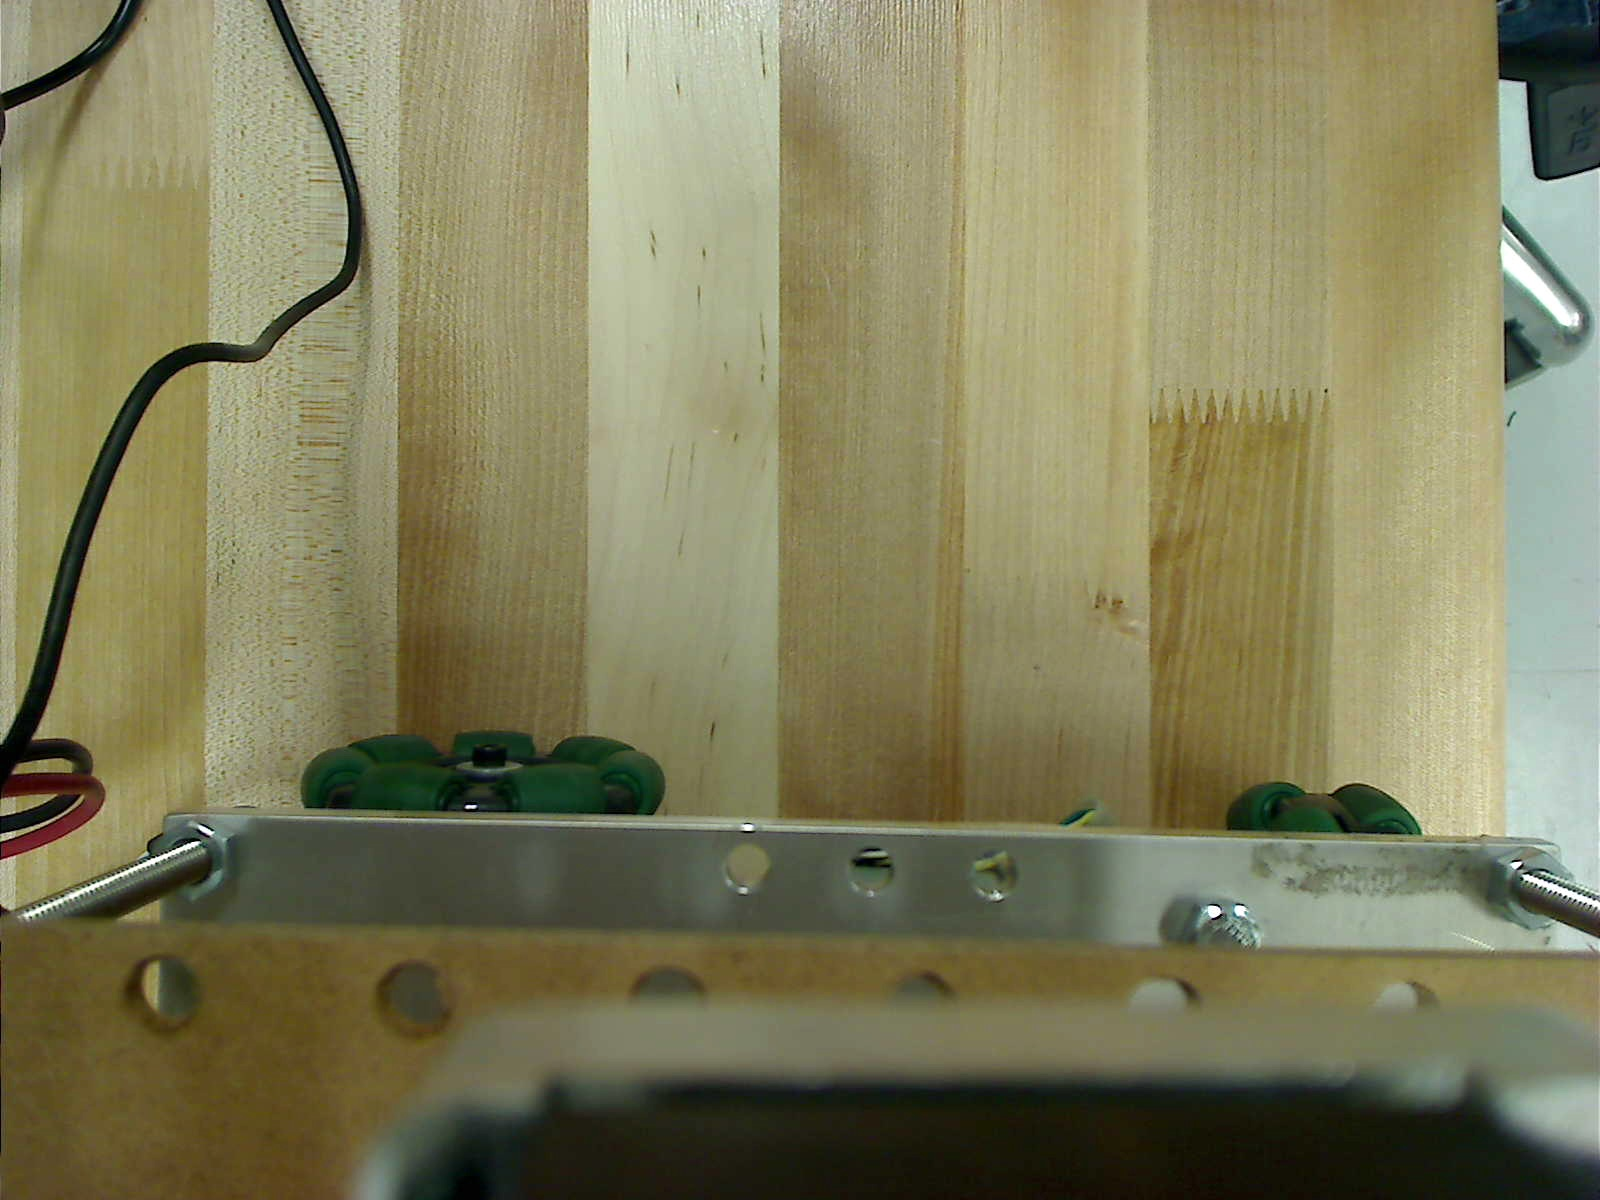
\includegraphics[width=0.95\textwidth]{fig/cam_embarquee.jpg}
   \caption{Vision au sol du robot � partir de la cam�ra embarqu�e}
   \label{f:cam_embarquee}
\end{figure}